\chapter{Discussion}
\label{chap:discussion}

\section{Overall reflection and experience}

Initially the group wanted to keep very high standards for code quality and professionalism. Although all still strove for this throughout the project they quickly fell behind schedule and sacrificed on professionalism in order to get working features and ensure scalability. The part of professionalism that suffered was mostly documentation of the process and unit tests. Part of why the documentation did not stand up to what was suggested in the project plan \ref{app:projectPlan}, was that the project plan template did not fit highly \gls{agile} workflows like what the group followed. The group followed \gls{scrum} and had documented sprint retrospective and sprint planning meetings, but the low communication threshold meant that most planning was done verbally and not through writing. It allowed for rapidly changing ideas and refactoring, but very little code that could be considered final and therefore not considered worth writing tests for. This will make it more difficult for potential \gls{opensource} developers to take over afterwards. Although it is unlikely that others will continue the project it still seemed like a valid compromise.

The low communication threshold meant that those working on relatively complex tasks would ask for a second opinion or ideas for potential solutions. This in turn meant that each group-member felt committed and prioritized the more advanced task. This most likely was beneficial and helped solve some of the tasks that could not have been solved by an individual. This also had the negative effects of down prioritizing less complex tasks that could easily give slight enhancements for the project and that the groups focus could slip. The groups would talk about project unrelated topics more than what was considered optimal and therefore had to spend more time than what was expected. Time log can be found in appendix \ref{app:timelog}.

It was often mentioned that progress was behind the schedule set in the project plan, although the schedule comment specifically mentioned that changes were expected and should be embraced. It is good that this pushed for quicker development, but it might also have harmed the scalability of the project and thereby also slowed it down by pushing for features when the plan was not fully formed.

The group was always aware that the project was complicated and required a lot of research and experimentation, but throughout the development it seemed that group members did not expect the same level of completeness. The product owner had at some occasions described the project as a research project, yet the supervisor mentioned that the project requirements should be written as hard requirements, something that conflicted with both the research based and agile nature of the project.

Overall impressions is as expected, the group knew the project was very ambitious and aimed more for an idea than a realistic goal as the learning outcome would be significant and it pushed the team to do better than what was realistic. It was hard work, but still very interesting and as a group there was a genuine belief that all members would want to continue developing the project after the thesis was finished.

\section{Use of Jira}
\newglossaryentry{toggl}{name={Toggl}, description={A time tracking app \cite{wiki:toggl}}}
Throughout the project the team used \gls{jira} for managing the backlog, sprints and the planning of tasks within these sprints. Some tasks at the start were quite large and required Full-Stack development, e.g. "As a user I would like to see classes parsed and visualized in 3D". These tasks are far too big, especially for the group who has very limited experience with the technologies used like Antlr and front-end development. The individual group members would also spend a whole week on the same task and this felt quite daunting after a couple weeks. The group then decided to make these tasks into epics and break them down into user-stories and sub-tasks that were more finely defined and segmented. This made the group members individually more motivated and made the development process feel less daunting, because a member could complete more tasks in a shorter period of time, therefore gain more satisfaction in seeing multiple tasks getting completed. The break-down of the tasks also had the added benefits in making the burn-down charts look more professional and would more accurately represent the work being done. Despite this underestimation was still a severe problem and some stories were not estimated due to Jira treating sub-tasks, stories and epics differently. The \gls{planningPoker} tool in \gls{jira} worked well for estimating stories, but had problems with subtask. Subtasks did not have an estimation field by default. This might be because \gls{jira} meant for them to be of trivial size. The team did not use them like that, but added an estimation field, however the \gls{planningPoker} tool did not pick this automatically. In general task estimations were greatly underestimated since it was difficult to see the full length of the task when the task was described orally.

To keep track of the time spent on each task, the group used \gls{toggl} and had it integrated with \gls{jira}. This was a slight problem as it required the administrators of our \gls{jira} instance. We also required the administrators for \Gls{git}Hub integration, project setup and team management. It seemed that \gls{jira}, although useful, was not the correct tool for our use case as it made it harder for the team to be independent.

There was also a problem with the \Gls{git}Hub integration as it did not allow for syncing of the issue tracker. This was a problem because the team wanted to handle the project as an \gls{opensource} project and wanted the issues publicly available. An alternative would be to use \Gls{git}Hub with plug-gins for issue tracking and estimations.

Decisions made during development were recorded using \gls{confluence}. The export can be found in appendix \ref{appendix:decisionLog}.

\section{Quality metrics and measures}
\newglossaryentry{taintPropogation}{name={taint propogation}, description={\todo{Find definition and site static analysis book from the course}}}
The quality metrics and measures were originally a very important aspect of the project, but were pushed back due to the complexity and how it required higher completeness of the Antlr parsing. The topic was researched and decided to focus on metrics mentioned in sub section \ref{subsection:SprintComplexParsingAndScopeVisual}.
For the \Gls{cyclomaticcomplexity}, counting the branching factor from conditionals and exit statements, seemed like something that could be done and would give a significant benefit, due to how it gives good representation of complexity on both function, class and project level. \href{https://github.com/SonarSource/sonarqube}{Sonarqube API} was considered as a way to add this into the project as mentioned in \ref{subsection:SprintComplexParsingAndScopeVisual}, but workload was too great and this is therefor still in development.

\Gls{connacensemetrics}, dealing with implicit connection within algorithms and between variables, was considered and seen as the Holy Grail of helpful statistics, but the complexity and difficulty of calculating this meant that it was decided that the group would not try to add it. The group do not even know if it would be possible to calculate connascence, it seem like something that would be more like a description in an oral conversation. For instance; the group could not find any reliable way to calculate the algorithmic connacence between a \gls{frontend} input validation and \gls{backend} validation. If the validation checks if a number is between 0 and 10, then the two validations can be written in different languages, have different names for the validated variable like "i" and "n". The group would have to know the \gls{url} the request is send to and the back-end redirects and how the back-end obtains the parameters. The group would have to know that it is a validation layer or that the validation is integrated into the behaviour. All in all the group do not even know if this is decidable. Despite this the group still found it useful for describing our own system and discussing potential refactoring. The team considered look into \gls{taintPropogation} techniques to get a better understanding of this. The team was fammiliar with \Gls{taintPropogation} through the software security course \cite{course:softSec} and knew it was outside the scope of this project.  

\section{IaC}
\newacronym{cicd}{CI/CD}{Continuous Integration and Continuous Deployment \cite{mabl:cicd}}
\newglossaryentry{puppet}{name={Puppet}, description={Is a configuration tool \cite{puppet}}}
\newglossaryentry{chef}{name={CHEF}, description={Is a configuration management tool \cite{chef}}}
As mentioned in \ref{sec:methodology}, it was initially going to be a greater focus on \gls{devops}. Sadly, due to the amount of work required for each feature and continual underestimation of time required for stories and issues, the team could not finish the \gls{cicd} features. \gls{cicd} were concepts the group really wanted and looked forward to using, but the lacking knowledge of the specific tools needed for this meant that it had to be cut short to focus on development. This was a necessary decision, but still one that was hard to make and one the team did not want to make. The team intended to use \gls{openstack} with \gls{hot} in such a way that one could automatically tear down and rise virtual servers as was recommended \cite{morris2016infrastructure}. The team is using \gls{openstack} and \gls{hot}, but the result could not be used in an automated process and the \gls{openstack} stack visualization shown in \ref{fig:serverNet} seem to indicate that that is wrongly configured.

\begin{figure}[H]
    \centering
    \includegraphics[width=\textwidth]{inc/images/DevOpsArchitecture.png}
    \caption{Server network architecture.}
    \label{fig:serverNet}
\end{figure}

The problem with using the stack for an automated process was that the team was unable to easily configure it together with \gls{jenkins} and \gls{docker}. The team knew that these services where often used together and with \gls{puppet} or \gls{chef} but were unable to find what tool was meant for what purpose. In the end the team used the \gls{hot} template tag to run script for installing docker that would in turn setup \gls{jenkins} master and slave. Then \gls{jenkins} could be configured to handle pushes to \gls{git} repository and update the slaves. As the server configurations were incomplete, it was easier for each group member to host and test on their local system instead.

If the server configurations had been completed, the setup could have been used to ensure test were run continuously and required for pull requests to be accepted. 

\section{Perspective on antlr}
\subsection{Overall reflection and experience}
Simple \Gls{antlr} workflow is explained in section \ref{sec:technicalBackEnd}. Each listener provides a context that represents a keyword within the file being parsed. The context is a sequential match of tokens. The number of tokens in a rule is the breadth of the context, whilst the depth of the context is number of nested tokens before you reach a fragment that is a leaf node and a character sequence. The form of a token is an alternative rule that match the context.  

At the beginning of the project the group decided to parse some basic parts of the code-base to get familiar with \gls{antlr}, without thinking much about making it a proper system. This way the group was able to come up with a working prototype in the first week of development, but as the development progressed, the code would not scale due to a few tasks that required huge nested-if blocks to deal with the depth of the contexts. The problem with if statements is explained in sub section \ref{subsection:parsingJava}.

To retain the professionalism in the code, the group needed to find out a better way to use \gls{antlr} for code parsing. Through research and experiments the group came up with 3 solutions over time to structure the \gls{antlr} part of the code-base:
\begin{itemize}
    \item Stack
    \begin{itemize}
        \item In the \gls{antlr} repository it was recommended to use stack like data-structure to process the code \cite{github:stackAntlr}. Since \gls{antlr} parses the code sequentially, a stack could be used to store what is being parsed and this solved our problem with understanding the scope of a context and by separating scopes. As \gls{antlr} runs on individual files, this approach was unable to identify scopes from different files. This was a problem with the C++ grammar as it sends include statements into a hidden channel. This meant that the group was unable to merge the different files into one project and connect structures and function calls declared in separate files.
    \end{itemize}

    \item Java Action
    \begin{itemize}
        \item Java Action was considered to help with context with large breadth and many forms where the context is known to have a wanted token. Actions would be for functionality to be added when entering or exiting a context. One could essentially say "When entering this scope; look for all instances of this token". It would return the wanted token no matter what sub-tree it was from alleviate the need to check what form each nested context has. It would do this by setting an \gls{antlr} listener to call an Action that is overwritten when entering or exiting a scope.
    \end{itemize}

    \item \gls{antlr} visitors 
    \begin{itemize}
        \item The \gls{antlr} visitor were recommended to gain more control in traversing the parse-tree and are usually used if only sub-trees are required to be parsed. The project required many different components of the codebase to be parsed and listeners were therefor the best option for us, where it will go through every node in the parse tree. This way the listeners could sequentially parse every built-in keyword or user defined names from every line on the code-base.
    \end{itemize}
\end{itemize}


\subsection{Decreasing cyclomatic complexity in antlr}

\tikzset{
    vertex/.style = {
        circle,
        fill            = black,
        outer sep = 2pt,
        inner sep = 1pt,
    }
}
\begin{figure}[H]

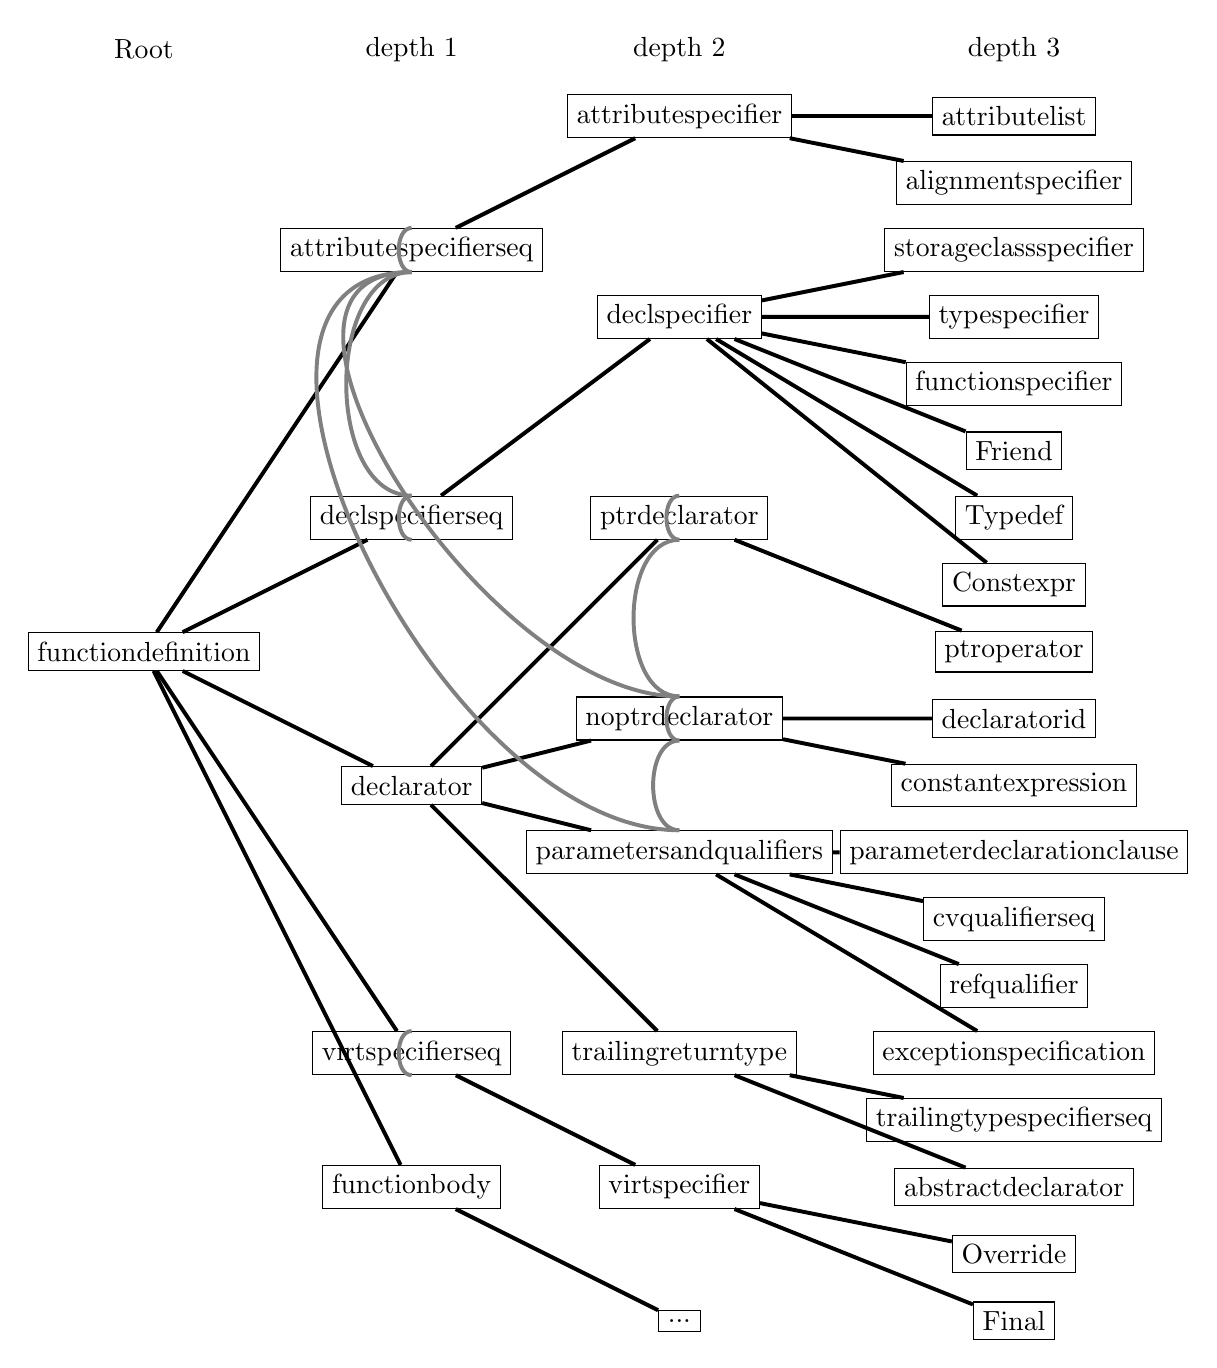
\begin{tikzpicture}[scale=0.85]
    % root
    \node at (0.0, 1.0) {Root};
    \node[draw] (funcDef) at (0.0, -8.0) {functiondefinition};
    
    %level1
    \node at (4, 1.0) {depth 1}; 
    \node[draw] (attribSeq) at (4, -2) {attributespecifierseq};
    \node[draw] (declSeq) at (4, -6.0) {declspecifierseq};
    \node[draw] (decl) at (4, -10.0) {declarator};
    \node[draw] (virtSeq) at (4, -14.0) {virtspecifierseq};
    \node[draw] (funcBody) at (4, -16.0) {functionbody};
    
    %root - level1
    \draw[line width=0.5mm,draw=black] (funcDef) to (attribSeq);
    \draw[line width=0.5mm,draw=black] (funcDef) to (declSeq);
    \draw[line width=0.5mm,draw=black] (funcDef) to (decl);
    \draw[line width=0.5mm,draw=black] (funcDef) to (virtSeq);
    \draw[line width=0.5mm,draw=black] (funcDef) to (funcBody);
    
    %level1 to exist
    \draw[line width=0.5mm,draw=gray] (attribSeq.south) to[in=180,out=180] (attribSeq.north);
    \draw[line width=0.5mm,draw=gray] (declSeq.north) to[in=180,out=180] (attribSeq.south);
    \draw[line width=0.5mm,draw=gray] (declSeq.south) to[in=180,out=180] (declSeq.north);
    \draw[line width=0.5mm,draw=gray] (virtSeq.south) to[in=180,out=180] (virtSeq.north);
    
    % level2
    \node at (8.0, 1.0) {depth 2};
    \node[draw] (attrib) at (8.0, -0.0) {attributespecifier};
    \node[draw] (declSpec) at (8.0, -3.0) {declspecifier};
    \node[draw] (ptrDecl) at (8.0, -6.0) {ptrdeclarator};
    \node[draw] (noptrDecl) at (8.0, -9.0) {noptrdeclarator};
    \node[draw] (param&qual) at (8.0, -11.0) {parametersandqualifiers};
    \node[draw] (trailReturn) at (8.0, -14.0) {trailingreturntype};
    \node[draw] (virtSpec) at (8.0, -16.0) {virtspecifier};
    \node[draw] (toMuch) at (8.0, -18.0) {...};
    
    %level1 - level2
    \draw[line width=0.5mm,draw=black] (attribSeq) to (attrib);
    \draw[line width=0.5mm,draw=black] (declSeq) to (declSpec);
    \draw[line width=0.5mm,draw=black] (decl) to (ptrDecl);
    \draw[line width=0.5mm,draw=black] (decl) to (noptrDecl);
    \draw[line width=0.5mm,draw=black] (decl) to (param&qual);
    \draw[line width=0.5mm,draw=black] (decl) to (trailReturn);
    \draw[line width=0.5mm,draw=black] (virtSeq) to (virtSpec);
    \draw[line width=0.5mm,draw=black] (funcBody) to (toMuch);
    
    %level2 to exist
    \draw[line width=0.5mm,draw=gray] (ptrDecl.south) to[in=180,out=180] (noptrDecl.north);
    \draw[line width=0.5mm,draw=gray] (ptrDecl.south) to[in=180,out=180] (ptrDecl.north);
    \draw[line width=0.5mm,draw=gray] (noptrDecl.north) to[in=180,out=180] (attribSeq.south);
    \draw[line width=0.5mm,draw=gray] (noptrDecl.south) to[in=180,out=180] (param&qual.north);
    \draw[line width=0.5mm,draw=gray] (noptrDecl.south) to[in=180,out=180] (noptrDecl.north);
    \draw[line width=0.5mm,draw=gray] (param&qual.north) to[in=180,out=180] (attribSeq.south);
    
    % level3
    \node at (13.0, 1.0) {depth 3};
    \node[draw] (attribList) at (13.0, -0.0) {attributelist};
    \node[draw] (alignmentspecifier) at (13.0, -1.0) {alignmentspecifier};
    \node[draw] (storageclassspecifier) at (13.0, -2.0) {storageclassspecifier};
    \node[draw] (typespecifier) at (13.0, -3.0) {typespecifier};
    \node[draw] (functionspecifier) at (13.0, -4.0) {functionspecifier};
    \node[draw] (Friend) at (13.0, -5.0) {Friend};
    \node[draw] (Typedef) at (13.0, -6.0) {Typedef};
    \node[draw] (Constexpr) at (13.0, -7.0) {Constexpr};
    \node[draw] (ptroperator) at (13.0, -8.0) {ptroperator};
    \node[draw] (declaratorid) at (13.0, -9.0) {declaratorid};
    \node[draw] (constantexpression) at (13.0, -10.0) {constantexpression};
    \node[draw] (parameterdeclarationclause) at (13.0, -11.0) {parameterdeclarationclause};
    \node[draw] (cvqualifierseq) at (13.0, -12.0) {cvqualifierseq};
    \node[draw] (refqualifier) at (13.0, -13.0) {refqualifier};
    \node[draw] (exceptionspecification) at (13.0, -14.0) {exceptionspecification};
    \node[draw] (trailingtypespecifierseq) at (13.0, -15.0) {trailingtypespecifierseq};
    \node[draw] (abstractdeclarator) at (13.0, -16.0) {abstractdeclarator};
    \node[draw] (Override) at (13.0, -17.0) {Override};
    \node[draw] (Final) at (13.0, -18.0) {Final};

    
    %level2 - level3
    \draw[line width=0.5mm,draw=black] (attrib) to (alignmentspecifier);
    \draw[line width=0.5mm,draw=black] (attrib) to (attribList);
    \draw[line width=0.5mm,draw=black] (declSpec) to (storageclassspecifier);
    \draw[line width=0.5mm,draw=black] (declSpec) to (typespecifier);
    \draw[line width=0.5mm,draw=black] (declSpec) to (functionspecifier);
    \draw[line width=0.5mm,draw=black] (declSpec) to (Friend);
    \draw[line width=0.5mm,draw=black] (declSpec) to (Typedef);
    \draw[line width=0.5mm,draw=black] (declSpec) to (Constexpr);
    \draw[line width=0.5mm,draw=black] (ptrDecl) to (ptroperator);
    \draw[line width=0.5mm,draw=black] (noptrDecl) to (declaratorid);
    \draw[line width=0.5mm,draw=black] (noptrDecl) to (constantexpression);
    \draw[line width=0.5mm,draw=black] (param&qual) to (parameterdeclarationclause);
    \draw[line width=0.5mm,draw=black] (param&qual) to (cvqualifierseq);
    \draw[line width=0.5mm,draw=black] (param&qual) to (refqualifier);
    \draw[line width=0.5mm,draw=black] (param&qual) to (exceptionspecification);
    \draw[line width=0.5mm,draw=black] (trailReturn) to (trailingtypespecifierseq);
    \draw[line width=0.5mm,draw=black] (trailReturn) to (abstractdeclarator);
    \draw[line width=0.5mm,draw=black] (virtSpec) to (Override);
    \draw[line width=0.5mm,draw=black] (virtSpec) to (Final);

    

\end{tikzpicture}

    \caption{CPP functiondefinition graph to depth 3}
    \medskip
    \small
    Straight lines show that the, right-hand side is contained within the left side.
    Curved lines show that something defined earlier or at the same level is also within the rule.
    \label{CPPFunctionDefinition}
\end{figure}


When parsing function definition, it became clear that the depth of the context caused significant complexity as on each level the form of the context had to be checked. This required significantly nested if structures.

The team solved this problem partially using a stack of models. A model represents a structure in the code-base; instance functions, classes, namespaces, etc. The model is added to the stack when it's scope is entered and removed after it has completed. This way the team was able to use specific listeners provided by \gls{antlr} to parse the specific fields for the model. 

With the stack more listeners could be implemented without worrying that a listener would be called at the wrong time and be added in the wrong scope. Instead of parsing function definition in depth, one could implement the relevant listeners within the context and they would automatically add their data to their parent model where the parent model was function definition.
In figure \ref{CPPFunctionDefinition}, implementing functiondefinition to enter a function model and implementing typespecifier to add its type to the parent would mean function model would have this without explicitly checking declspecifierseq and declspecifier. 

Implementation of listeners in the object-oriented design created a lot of dependency relationships which increase \gls{connacensemetrics} of the code-base. As figure \ref{CPPFunctionDefinition} shows every node in depth is dependent on its parent node, in most cases some nodes share the same parent node. This make it very difficult to figure out what listener could be executed next. This was still considered a good alternative as it removed a lot of \gls{cyclomaticcomplexity} and meant that more of the parsing burden was dealt with by \gls{antlr}. 

Another solution for this could be using \gls{antlr} visitors, where visitors gives much more control on which token to visit. This way could exclude irrelevant sub-trees and only visit the information about a specific model. Due to time limitation, visitors were not experimented with but this could be useful for future refactorings.

\subsection{Use of regex}
\newglossaryentry{regularExpression}{name={regular expression}, description={A sequence of characters that define a search pattern \cite{wiki:regex}}}
\newacronym{regex}{regex}{\Gls{regularExpression}}

Handling function calls was difficult as in Java and C++, the call can be called on an object and that object can in turn be called on any other object recursively. The grammar did not easily as the languages are very versatile with what an object might be. To bypass the difficulty of using \gls{antlr} for this purpose, the group decided to use \gls{regex}. The \gls{regex} was used to split the call on "." and "->" that delimited the different objects while other string operations were used to remove the body of some brackets. \Gls{regex} could not remove the content of brackets correctly as they could in turn contain brackets and \gls{regex} can not handle \gls{recursion}. The content of brackets were removed to make it easier to identify the associated function. This approach would not scale in the long run and is likely to create problems. The problems that can arise come from how this approach prevents \gls{antlr} from taking care of of the recursive structure and niche aspects of the languages that the team has not considered. Removing the body also prevents the system from knowing what overloaded function is being called. Using the \gls{antlr} build in features would be preferable in the long term, but would require significantly more work. 


\Gls{regex} approach could also be used to parse function pointer assignments as this was a problem due to use of symbol "*" as a pointer and was also used as a multiplication sign. This made it impossible for the team to differentiate between pointer assignment and multiplication expression. A long term solution to this problem could be updating the grammar file with a rule for pointer assignments, but this was not done since it would require in-depth understanding of grammar files. Function pointers were dropped due to time and parsing for other simple structure that yet had to be done.


\section{Perspective on REST and WebSocket}
As mentioned in sub section \ref{subsection:golang}, \gls{rest} requirement of the project had to be relaxed, \gls{websocket} was a necessary decision to take and integrate into the system. \Gls{websocket} are built-in to \gls{js} and a easy-touse library for Go, made it quick to set up and worked well for our needs.

\Gls{websocket} is a different protocol that uses \gls{http} requests to request a \Gls{websocket} connection and then switches over to \Gls{websocket} protocol if server allows. This allows messages to be sent back and forth over 3 different channels, "open", "close" and "message". The "open" channel is for when the \Glspl{websocket} opens, "close" is for receiving shutdown message for the connection and "message" is for any information that needs to be sent. 

One solution to improve the \gls{rest} portion of the \gls{api} is to offer \Glspl{websocket}, along with a \gls{rest} \gls{api}, which will give next to no information about the parsing progress, but returns the same result.

The use of \gls{websocket} in Go led to very huge functions and this resulted in decreased readability of the endpoints. Huge functions were the side effect of error handling of \gls{websocket}. To improve readability the team could break the the functionality of the endpoint into multiple small functions.

One mitigation for the massive amount of error handling would be to use a concept called middleware. This is when you have code that is executed before or after any given code snippet for a specific reason. For example one could wrap a log-in code in middleware that would write to a log-file that that specific user tried to log in, then run the log-in functionality and maybe after state in the log-file that the log-in was successful. As well as logging it could be used for prepping or extracting input to sensitive functions ensuring no taint-propagation and injections, as well as error handling.

\section{Perspective on Graphics systems}
\subsection{Overall reflection and experience}
Selection of a graphics system was relatively easy, the whole group had experience with OpenGL from the Graphics programming course and \gls{webgl} is closely related. Everyone already knew the details on how to draw in 3D, but since it was a new language the group didn't have much experience in, the group setup a workshop to familiarize our selves with \Gls{js} and \gls{webgl}. The group also found THREE.js which is a well-known and well-used graphics framework in \Gls{js}. THREE.js handles \gls{webgl} automatically, was easy to use, contains ready made shapes called geometries and have a lot of support functionality like vector classes with built-in math. The group therefore decided to use THREE.js.

The project required to show information and interact-able \gls{ui}, for this reason the group researched different \gls{ui} Libraries/frameworks and 2D Drawing libraries and found PixiJS, TWO.js, dat.GUI and ImGUI-JS.

\subsection{Choice of graphics framework}
Using THREE.js then meant that the graphics handling was not a problem, but there were still a problem with using the parsed code-base to create the 3D representation. This was handled in \Gls{js}, although later it seemed like parts of it could be handled by the \gls{backend} and allow for an improved web \gls{api} and better caching opportunities. 

\subsection{Choice of UI framework}
The group thought about creating a custom \gls{ui} system using PixiJS or TWO.js instead of using other existing libraries. This seemed like a lot of management and adjustment work, considering it would only be used for the visualization. 

dat.GUI is a pure \Gls{js} and HTML \gls{ui} Library. Although it seems easy to use and could possibly work, it seemed too simple from available examples. This would require large amounts of configuration code and would stretch the library's capabilities, which wasn't really desired. Only scenarios where "dat.GUI" would fit well is for a settings or configurations drop-down menu.

ImGUI-JS is a 3rd party library and must work in unison with ImGUI, but the difference from TWO.js and PixiJS is that ImGUI-JS wrappes ImGUI, so in-effect they're one library and this made it very difficult to integrate, therefore lot of time went into making it work properly, but the group didn't have to get two libraries to work at the same time. Another benefit of ImGUI is that the \gls{ui}-elements exists inside windows which is by default movable and scale-able and results into a very customize-able \gls{ui} layout out of the box if this is wanted.

\subsection{Choice of Application Lifecycle Framework}
\newacronym{alf}{ALF}{Application Lifecycle Framework}

The group considered to use framework for \gls{frontend} development because use of framework is often recommended, especially when using \Gls{js} due to the way it handles scopes. The supervisor recommended multiple frameworks such as POLYMER.js, VUE.js, AngularJS and REACT.js. The project is a web-based application which has only two HTML pages and most of the \gls{frontend} deals with graphics.

Considering this the team later realized that there was no need for it. Most \gls{alf} are not designed for graphics focused \gls{js} or for this application. It could restrict and require time to learn without giving any significant benefits.

\subsection{Use of Force Directed Graph library}
There are a multitude of libraries out there that handles \gls{fdg} quite good like \href{https://www.npmjs.com/package/3d-force-graph}{3d-force-graph} and \href{http://getspringy.com/}{Springy.js}, but non of these libraries allowed for individual link strengths. They only have a single global setting for all attractive links, and the reason this was wanted was due to the different data-structures being more or less attracted to other certain data-structures. Therefore it was decided to implement it. 

\subsection{Graphics system refactoring}
The 3D representation creation was changed multiple times but not fully refactored so it still contains code that should have been deprecated, removed or changed to fit the rest of the system. Some of these changes were made late in the project when time-constraints were causing problems. The time-constrains meant that proper refactoring would not improve the velocity of the team and were therefore not prioritized.

\section{Perspective on FDG}
\subsection{Overall reflection and experience}

The code-base visualization had to be intuitive and able to handle both large and small data-sets without any manual adjustment by the user or administrator. A \gls{fdg} seemed like a natural choice for automatically adjust the layout based on the scale and composition of the code-base. It also seemed natural to use the scoping in object oriented programming to hide or reveal details based on what the user was looking at.

As this was the first time the group had used \gls{fdg}, it was a surprise how flexible the literature was about the implementation specification. The literature helped establish a few terms:

\begin{itemize}
    \item Node - A representation of code-base structure with positional data and metadata requiered by \gls{fdg} to update position.
    \item Energy - relating to the total energy in the system and what the \gls{fdg}'s goal was to minimize.
    \item Attractiveness - metadata of node relating to how much energy is required to keep it apart from one other node.
    \item Repulsiveness - metadata of node relating to how much energy is required to keep it close to one other node.
    \item Links - metadata of node, A map of all repulsive and attractive forces to all other nodes.
    \item Gravity - A global force affecting all nodes, pulling them towards a defined center.
\end{itemize}

\subsection{Detailed experience on refactoring of FDG}
The Force Directed Graph (FDG) is probably the part in the program that caused the most problem when trying to expand on it and refactor it.
It started off as a prototype with limitations:
\begin{itemize}
    \item Assumed no nested structures as output.
    \item Assumed a global center that all structures should gravitate towards to keep the graph centered.
    \item Assumed an initial repulsion from one structure to another, that's not related and of equal strength.
    \item Assumed the repulsive forces was negative by the algorithm.
    \item Assumed all repulsive forces were set as -1 by the parsing.
    \item Assumed a connection or attraction from structures based on nested structures in input.
\end{itemize}

The \gls{fdg} used Inverse-square-law to calculate force based on repulsiveness and Hooke's law to calculate a force from attractiveness. All the nodes were parsed from the initial nested code-base structure in pre-order and stored in a single array within the \gls{fdg} object.
The initial structure allowed for relatively simple parsing and well understood and fairly versatile structures. Initially it was desirable for nodes to contain minimal information and only the information required by \gls{fdg} as this would improve the object oriented model and minimize the amount of data being passed around. The desire to keep nodes minimal was lessened when the group looked into \gls{js} as a "Share by Calling" language. 

When it came to changing \gls{fdg} to allow for nested structures as output, it soon became clear that large portions would have to be changed. The wish was to have a system that would be streamline and versatile. This meant to change array containing all the nodes into a generic tree that more closely represented both the input data and output data. It was required to change the single array approach as allowing for nested outputs meant the \gls{fdg} would have to run on each nested part separately. Changing the array proved complicated, as links were added while parsing the input and used the index in the array to identify the other node, with a tree the index would have to be calculated and kept constant. It was thought that keeping the index constant could only be done by parsing the input level-order or pre-order, and this would not allow for nested output as the size of each node was dependent on its children. Therefore the parsing was done post-order and contained a local index that could be used to calculate the global index in the tree when connected to the root. This result is described in \ref{subsubsec:recuriviryOfNode}. This assumption turned out to be wrong, and giving the nodes a global index when building the tree would have been beneficial.

The local to global calculation caused a lot of confusion and significantly increased complexity. The new system had the same cyclomatic complexity as before, keeping conditionals essentially the same, but increased the use of complicated \gls{recursion} and had a high connacance with the removed array through the global index.

Although there were made mistakes during the refactoring and it increased the complexity, it was still beneficial. benefits of using the tree structures were evident as the group could run \gls{fdg} on each node separately with zero vector as their origin as inputting that into Three.js \gls{scenegraph} to handle offsets and potential navigation. From parsing in Java, through models in Golang, parsing in \gls{js}, \gls{fdg} for calculating position and to Three.js \gls{scenegraph}, the core data is always handled with a tree structure. This means there is a high level of consistency throughout the system but also an implicit connacance that means if the structure is changed in Java then all other parts will also have to be changed.

\section{"sloccount" vs "Kloc" vs "wc -l"}
One of the simplest complexity metrics to add was \gls{loc} and was added as a first, simple metric. Sloccount, kloc and wc are tools that can get the \gls{loc}. wc was chose. 
wc is a linux command line tool to read words, newlines and bytes and prints out the result to standard output channal. wc is language independent meaning it can take any language file as an argument. It can also read only the specified lines within the files by giving "-l" flag when executing. This worked for our purpose and therefor used to fetch the implementation from source code files. The other alternatives were considered because wc would not be able to distinguish between comments, code or empty lines, but the other alternatives had the same limitations or would not support enough languages for our purpose. 

\section{Platform for the product}
The reason of choosing web as the platform for the the system was it to be cross-platform and so that any user could easily access the system from anywhere. Also The team did not have much experience in the web-technology therefor it was a good opportunity to implement the system as web-service.
\gls{js} is the technology the team didn't not have much experience with and become a problem to scale as responsibilities of \gls{frontend} increased over time.

\section{Post-phoning / removing userstory allowing user to submit lexer files}
There were an idea early on that the user would be able to input a lexer file for any language and be able to use it to visualize projects with-in that language. It became clear very quickly the more we worked with \gls{antlr} that this feature was not going to be integrated. As described above, the listener files are generated and language specific, and each of them has different names for same listener, etc.
So to integrate them we have to either inject the new code in during runtime which is far beyond the 
So it was decided to drop this functionality due to the shear size of the feature which on it's on can be counted as a bachelor if not even more.